\chapter{Implementation}

%Explain what you did to implement your solution, problems that occurred and how you fixed them. 
%If they are interesting, include some relevant parts of the implementation (most relevant pieces of code and so on). 

\section{Communication Protocols}


Centralized pool and robots need to share task information with each other. There are some basic requirements for communication: firstly,
robot should initiate the communication once it has finished all task in task queue and get free. This is solved by assigning robot controller as ROS service client and centralized pool as ROS service server.
This method saves unnecessary communication cost by avoiding keep tracking the current position, availability and states of all robots.
Secondly, robot should forward sensor data to centralized pool while processing a task. This is solved by assigning robot controller as ROS action server and centralized pool as ROS action client.
As is shown in \ref{fig:comminication}, an efficient communication protocols is designed. 

\subsection{Message about Measurement}
\label{sec:measurement_message}
When a robot pass by a door, it will receive messages from sensor. 
In order to save resources, instead of a system enviroment in real life, a door simulator ROS node is used to publish all measurement result for all doors. The message formart is shown in Table \ref{tab:sensor_message} 
The measurement results(opened and closed) are created according to the "open possible" column in the "open possibilities" table (Figure \ref{fig:database_er}).

\begin{table}[htb]
\centering
\begin{tabular}{|c|c|c|c|c|} 
\hline
Door ID  & Position& Timestamp & Measurement Result \\
\hline\hline
1&(-18.5,5.2) & 2020-06-01 9:00:02 & Door opened \\ [1ex] 
\hline
\end{tabular}
\caption{Measurement Message Format and Example}
\label{tab:sensor_message}
\end{table}
	

\subsection{Message about Task}
\label{sec:task_message}
Four types of message are defined: 
(1)Task request message(Table\ref{tab:request_message}); (2) Task goal messages(Table \ref{tab:goal_message}); (3) Task feedback message (Table \ref{tab:feedback_message}); (4) Task result message (Table \ref{tab:result_message}). 

\begin{figure}[htbp]
    \centering
    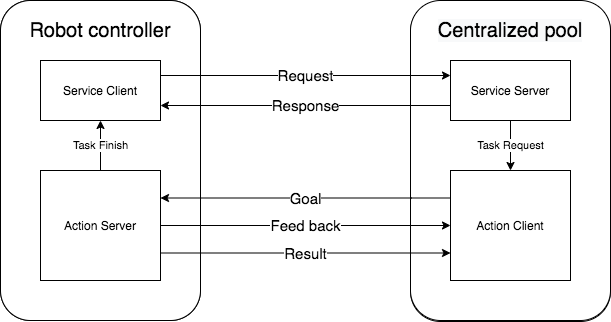
\includegraphics[width = 0.7\textwidth]{content/images/ch4/robot_pool_comminication.drawio.png}
    \caption{Communication between Robot and Centralized Pool}
    \label{fig:comminication}
\end{figure}

\begin{table}[htb]
\centering
\begin{tabular}{|c|c|c|} 
\hline
Battery & Pose & Robot ID\\
\hline\hline
93	&(2,4)	&1 \\ [1ex] 
\hline
\end{tabular}
\caption{Request Message Format and Example}
\label{tab:request_message}
\end{table}

\begin{table}[htb]
\centering
\resizebox{\textwidth}{!}{
\begin{tabular}{|c|c|c|c|} 
\hline
Task id[] &Task type & Target id & Goal[] \\
\hline\hline
1& Gather Environment Info & 9	& (-1.5,5.2) 2020-06-01 9:00:00 \\
\hline
[3,4]	& Execute task & 21, 22	& (-24.0,12.0), 2020-06-01 9:02:00 (-21.0,12.0) 2020-06-01 9:02:00 \\
\hline
5	& Charging	& 17	&(0.0,5.0), 2020-06-01 9:04:00 \\ [1ex] 
\hline
\end{tabular}}
\caption{Action Goal Message Format and Example}
\label{tab:goal_message}
\end{table}

\begin{table}[htb]
\centering
\begin{tabular}{|c|c|c|c|} 
\hline
Robot id & Door id & Measurement time & Measurement result \\
\hline\hline
1	& 3	& 2020-06-01 9:00:03 & Door open \\ [1ex] 
\hline
\end{tabular}
\caption{Action Feedback Message Format and Example}
\label{tab:feedback_message}
\end{table}

\begin{table}[htb]
\centering
\begin{tabular}{|c|c|c|} 
\hline
Task id	& Task type	& Result\\
\hline\hline
1 & Gather Enviroment Info & Success \\ [1ex] 
\hline
\end{tabular}
\caption{Action Result Message Format and Example}
\label{tab:result_message}
\end{table}


\begin{table}[htb]
\centering
\begin{tabular}{|c|c|c|} 
\hline
Robot ID & Battery Level \\
\hline\hline
1 & 93 \\ [1ex] 
\hline
\end{tabular}
\caption{Message to Charging Station}
\label{tab:message_to_charging_staion}
\end{table}

\subsection{Message about Charging}
  
Figure \ref{tab:message_to_charging_staion} shows the message a robot sends to Charging station when it arrives charging station's position.


\begin{figure}[htbp]
    \centering
    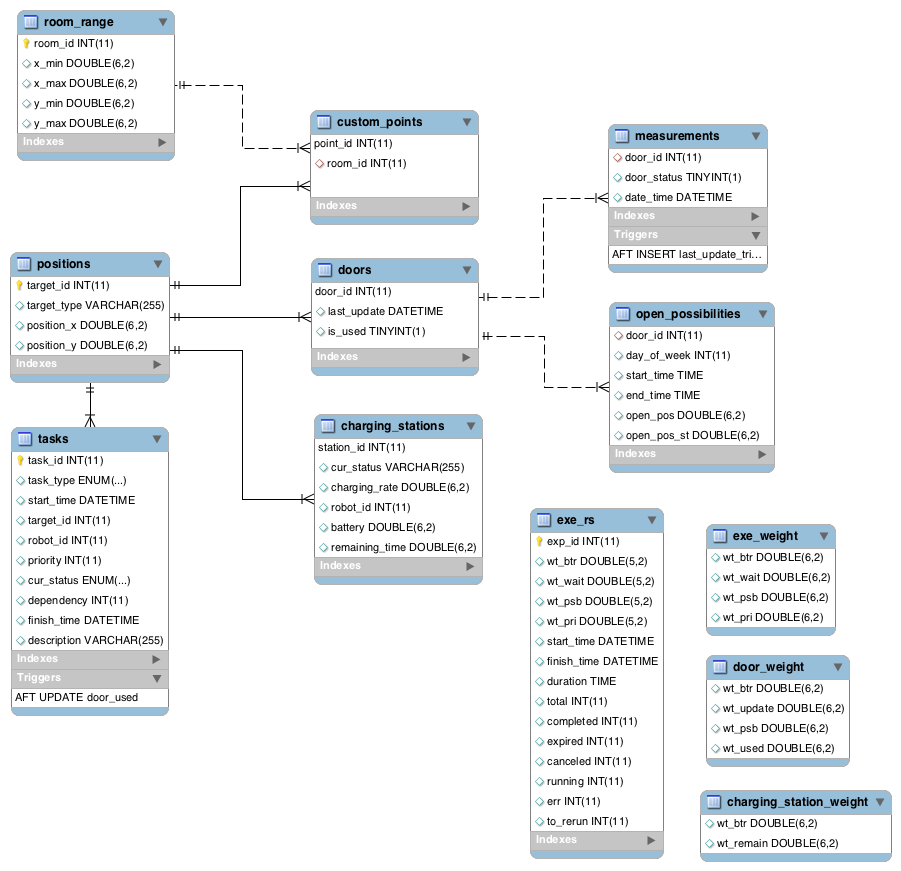
\includegraphics[width = 0.7\textwidth]{content/images/ch4/database_er.png}
    \caption{Database Entity Relationship Diagram}
    \label{fig:database_er}
\end{figure}


\section{Database}
The centralized pool keep information it requires, to make decisions. Figure \ref{fig:database_er} shows the relationship between entities. Following are explanations of some tables.
\begin{itemize}
	\item \textsl{Table doors.} Table doors stores enviroment information. In table doors, the is\_used column will be updated when an Enviroment-task to this door is updated. The last update will be updated when the centralized pool receive a new measurement result. 
	\item \textsl{Table open\_ossibilities.} Table open\_ossibilities is based on the statistic of door measurement in a specific time period of each working day. These two table will be updated when centralized pool receive a new measurement result. 
	\item \textsl{Table exe\_rs.} Table exe\_rs stores experiment result while table exe\_weight, table door\_weight and table charging\_station\_weight stores weight values for experiment. Chapter 5 introduces the details of experiment.
	\item \textsl{Table costum\_points.} When user gives the system a task, the target point of this task will be stored in position table, and a target\_id will be generated.  This target\_id will be stored in custum\_point table. 	Additionally, with the information in room\_range table, the system will recognize which room does the point belong to and write room\_id column in costom\_points table.
\end{itemize}


\section{Procedure}
As stated in the Chapter 3, the goal of task scheduling is finishing all tasks as soon as possible while keep the cost as low as possible. 
The task assignment and execution happends at two level. \cite{Ivan2017} the task and the path planner solves a planning problem. It takes and occupancy grid, a specific robot and a set of task specifications, and generates trajectorys for each task. According to those trajectorys and task specifications, the task with the lowest cost is assigned to robot.
At the dynamic level, after each robot receive a task, it runs a navigation stack to execute this task stepwise. Each robot computes a local trajectory but takes into account dynamic obstacles.
The process of the robot task allocation system is as follows.


\begin{figure}[htbp]
    \centering
    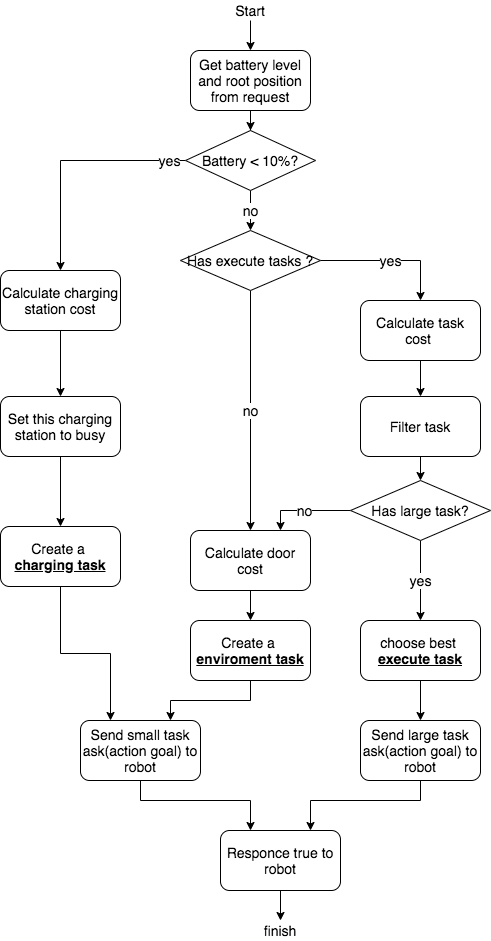
\includegraphics[width = 0.7\textwidth]{content/images/ch4/centralized_task_select.drawio.png}
    \caption{Centralized Pool Task allocation}
    \label{fig:centralized_task_allocation}
\end{figure}
\subsection{Centralized Pool}

\paragraph{Task Allocation}
When the centralized pool receives a task request (Table \ref{tab:request_message}) from robot, it performs task allocation. The task allocation algorithm is discussed in Section \ref{sec:task_allocation}. The process of task allocation is shown in Figure \ref{fig:centralized_task_allocation}. 
\begin{enumerate}
	\item When the battery of robot belows 10\%, the centralized pool create a charging task to the charging staion with the lowest cost.
	\item When the battery of robot aboves 10\%, the centralized pool loads execute-tasks in database, then combine small tasks with dependencies into large tasks, finally calculates task costs and select one large task with the lowest cost. 
	\item If there are no suitable tasks, a gather-enviroment-task to the door with the lowest cost is generated. 
\end{enumerate}
The difference between task is discussed in Section \ref{sec:task_specifications}. The output of the task allocation includes: task ID, goal coodinate, timestamp and selected robot ID. The task is sent to the selected robot, and the robot performs the tasks.

\paragraph{Handle Task Feedback.}
When the centralized pool receives a task feedback (Table \ref{tab:feedback_message}) that contains a new measurement result from robot, it will add a record in measurement table and update "open possibilities" table in database.

\paragraph{Handle Task Result.}
When the centralized pool receives a task result (Table \ref{tab:result_message}), it updates "tasks" table (Figure \ref{fig:database_er}). The failed "execute tasks" will be reused while the failed others will be marked as "Cancel" or "Error"(Figure \ref{fig:centralized_task_handle}).

\begin{figure}[htbp]
    \centering
    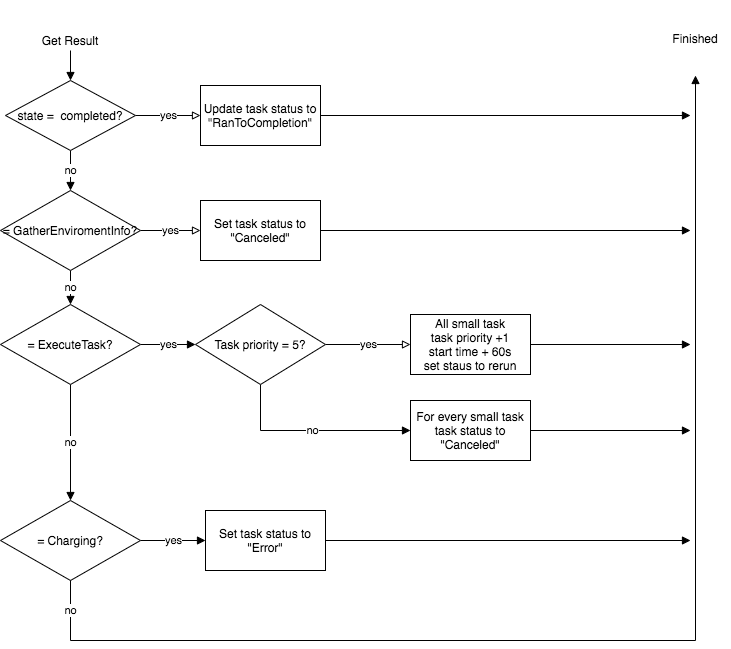
\includegraphics[width = 0.7\textwidth]{content/images/ch4/centralized_task_result.drawio.png}
    \caption{Centralized Pool Handle Task Result}
    \label{fig:centralized_task_handle}
\end{figure}


\subsection{Robot}

\begin{figure}[htbp]
    \centering
    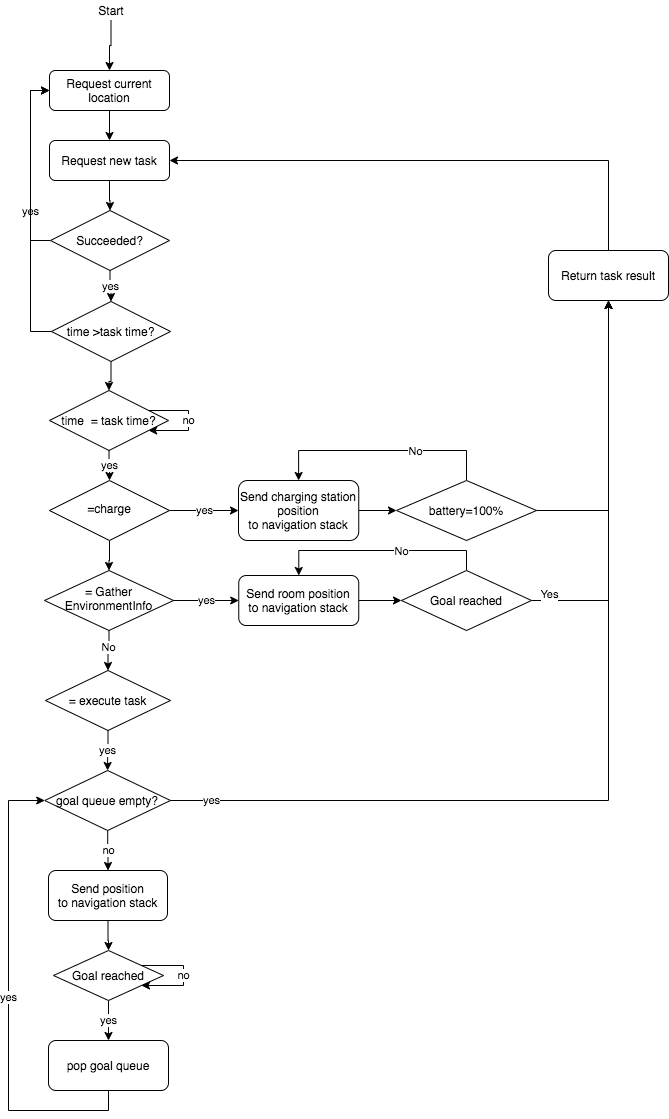
\includegraphics[width = 0.7\textwidth]{content/images/ch4/robot_process_task.drawio.png}
    \caption{Robot Process Task }
    \label{fig:task_process_robot}
\end{figure}

\paragraph{Robot Process Tasks}
When the task queue(Figure \ref{fig:system_architecture}) in a robot is empty, robot requests a new task. If the robot gets a "charging task", it will move to the position of charging staion(Figure \ref{fig:positions_door_station}) and interact with charging station node (Section \ref{sec:charging_station}).
When a robot gets an "execute task" which is a large task, it will move to all goals in order.
When a robot gets a "gather enviroment information" task, it will move to the door's position.
During task processing, the timer checks periodically the status of navigation stack. If any errors occurs, the robot send a "failed" result with description to the centralized pool.  
When task compltes without error, the robot will send "Succedded" result to the centralized pool.


\begin{figure}[htbp]
    \centering
    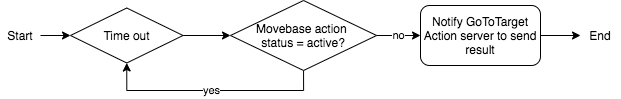
\includegraphics[width = 0.7\textwidth]{content/images/ch4/robot_timer.drawio.png}
    \caption{Robot Timer}
    \label{fig:robot_timer}
\end{figure}

\begin{figure}[htbp]
    \centering
    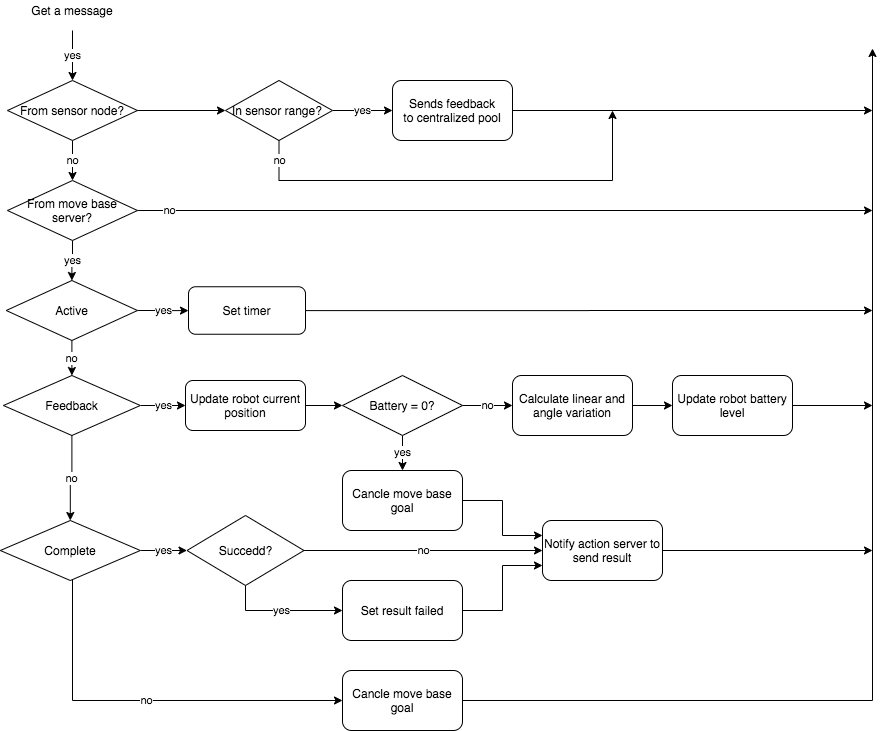
\includegraphics[width = 0.7\textwidth]{content/images/ch4/robot_message.drawio.png}
    \caption{Robot Hanlde Message}
    \label{fig:robot_handle_message}
\end{figure}

\paragraph{Robot Handle Messages}
While a robot is processing a task, it listens to door sensors and forwards measurement result to the centralized pool. 
Besides sensor messages, it receives messages from move\_base node. The details of robot message handling is shown in Figure \ref{fig:robot_handle_message}.

\subsection{Charging Station}
\label{sec:charging_station}
The charging station consist of a charging station node and "charging station" table in database (Table \ref{fig:database_er}). 
When a robot arrives the position of charging staion, it will start interacting with charging station node. Once the charging station receives robot's information(Figure \ref{fig:charging_station_message}), it changes its state to "charging"(Figure \ref{fig:charging_station_state_machine}) and increase on its value on "battery level"colum and increase its value on "remaining time"colum in database(Figure \ref{fig:charging_station_event}).  Once charging finished, its status will be set "charging finish". Once robot leaves charging station, its status will be set "free". 


\begin{figure}[htbp]
    \centering
    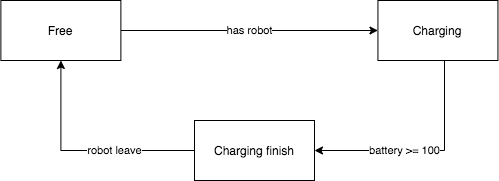
\includegraphics[width = 0.7\textwidth]{content/images/ch4/charging_station_state_machine.drawio.png}
    \caption{Charging Station State Machine}
    \label{fig:charging_station_state_machine}
\end{figure}

\begin{figure}[htbp]
    \centering
    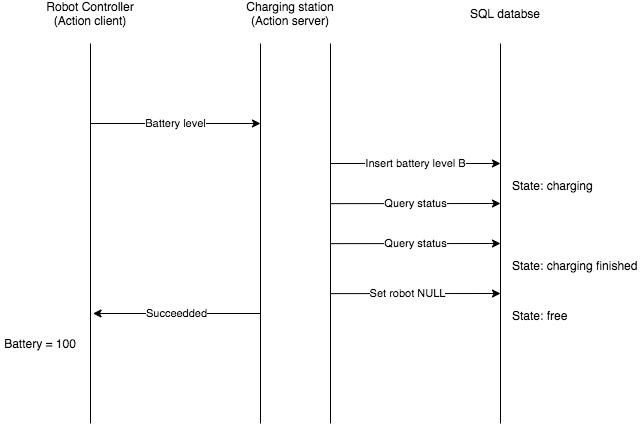
\includegraphics[width = 0.7\textwidth]{content/images/ch4/charging_station_message.drawio.png}
    \caption{Charging Station Message}
    \label{fig:charging_station_message}
\end{figure}

\begin{figure}[htbp]
    \centering
    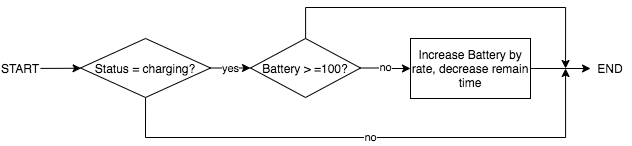
\includegraphics[width = 0.7\textwidth]{content/images/ch4/charging_station_charging_event.drawio.png}
    \caption{Charging Station Scheduled Charging Event}
    \label{fig:charging_station_event}
\end{figure}

\section{Unit Test}
Unit tests test each part of the program that the individual parts are working correctly. In this program, Google test is used to test system module such as task allocation module, execution modules and so on. 

